\documentclass{article}

% Add packages here
\usepackage{amsmath,bm}
\usepackage{color,soul}
\usepackage{graphicx}
\usepackage[margin=1.0in]{geometry}


\title{APPM 5460 Proposal - Don's Sections}
\author{Luke Bury \& Don Kuettel}

\begin{document}
\maketitle

\section*{Introduction}
This proposal aims to investigate homoclinic orbits in the dynamical system known as the Circular Restricted Three-Body Problem (CR3PB). The CR3PB, further described in the following section, is a classical astrodynamics problem that has been studied for over 200 years and contains a plethora of interesting dynamical phenomena, including homoclinic orbits. 

In mathematics, a homoclinic orbit is defined as a trajectory of a flow of a dynamical system which joins a saddle equilibrium point to itself. More precisely, a homoclinic orbit lies in the intersection of the stable manifold, $W^s(p)$, and the unstable manifold, $W^u(p)$, of an equilibrium. Figure \ref{f:homoclinic_example} shows an example of a simple, two-dimensional homoclinic orbit about the saddle equilibrium point $p$. As the figure shows, as time approaches either negative or positive infinity, the homoclinic orbit will approach $p$. 

\begin{figure}[h!]
    \centering
    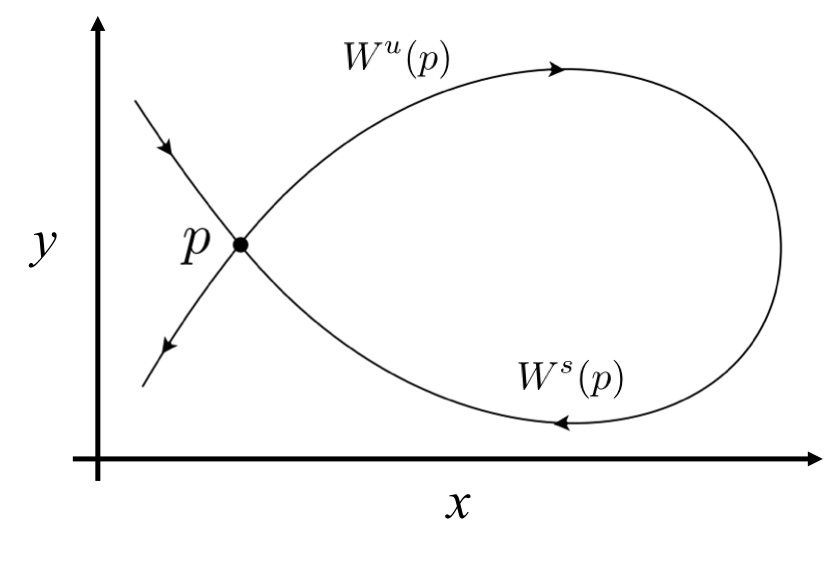
\includegraphics[width=4in]{figures/homoclinic_orbit.png}
    \caption{This figure depicts a 2D homoclinic orbit.}
    \label{f:homoclinic_example}
\end{figure}

Homoclinic orbits, first discovered by Henri Poincaré in the 1885 Acta Mathematica competition sponsored by King Oscar II of Sweden, play an important role in the chaotic behavior of a dynamical system. Lying on the intersection between a stable and unstable manifold of the same equilibrium point, or orbit, the geometry of homoclinic orbits (i.e., the geometry of the manifold intersection) offers a way in which simple local information can be extrapolated to complicated global behavior. This proposal looks to study Poincaré's work on homoclinic orbits and use that knowledge to find examples of homoclinic orbits in the CR3BP.

\end{document}